% ============================================================================
% Coordonnees du barycentre dans un repere
% Extrait de la fiche : Barycentres et lignes de niveau (classe de 1ere D)
% Necessite \usepackage{tikz} et \usetikzlibrary{calc} (charges par le fichier principal)
% ============================================================================
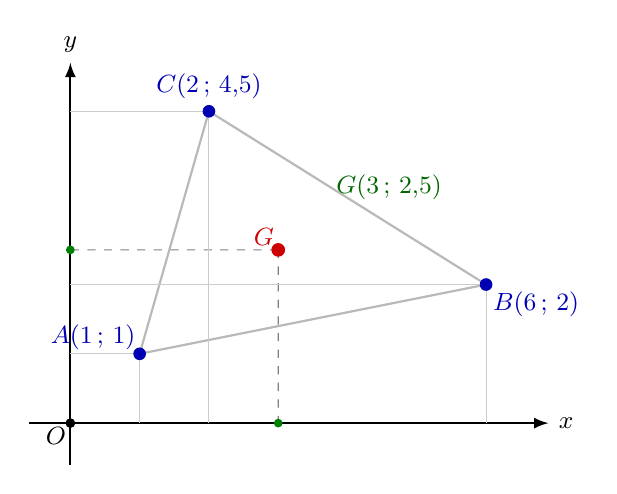
\begin{tikzpicture}[scale=0.88,>=latex]
  \draw[->,thick] (-0.6,0) -- (6.9,0) node[right,font=\small] {$x$};
  \draw[->,thick] (0,-0.6) -- (0,5.2) node[above,font=\small] {$y$};
  \coordinate (A) at (1,1); \coordinate (B) at (6,2); \coordinate (C) at (2,4.5);
  \coordinate (G) at (3,2.5);
  \draw[gray!55,thick] (A) -- (B) -- (C) -- cycle;
  \draw[dashed,gray] (G) -- (3,0); \draw[dashed,gray] (G) -- (0,2.5);
  \draw[gray!40,thin] (1,0) -- (1,1); \draw[gray!40,thin] (0,1) -- (1,1);
  \draw[gray!40,thin] (6,0) -- (6,2); \draw[gray!40,thin] (0,2) -- (6,2);
  \draw[gray!40,thin] (2,0) -- (2,4.5); \draw[gray!40,thin] (0,4.5) -- (2,4.5);
  \fill[blue!70!black] (A) circle (2.6pt) node[above left=-2pt,font=\small] {$A(1\,;\,1)$};
  \fill[blue!70!black] (B) circle (2.6pt) node[below right=-1pt,font=\small] {$B(6\,;\,2)$};
  \fill[blue!70!black] (C) circle (2.6pt) node[above=1pt,font=\small] {$C(2\,;\,4{,}5)$};
  \fill[red!80!black] (G) circle (2.8pt) node[above left=-2pt,font=\small] {$G$};
  \fill[black] (0,0) circle (2.0pt) node[below left=-2pt,font=\small] {$O$};
  \fill[green!50!black] (3,0) circle (1.8pt); \fill[green!50!black] (0,2.5) circle (1.8pt);
  \node[green!40!black,font=\small] at (4.6,3.4) {$G(3\,;\,2{,}5)$};
\end{tikzpicture}
